%! Tex program = xelatex

\documentclass{article}
\usepackage[left=2cm, right=2cm, lines=45, top=0.8in, bottom=0.7in]{geometry}

% \usepackage[utf8]{inputenc} % 用于指定文件的编码格式  
% \usepackage[fontset=ubuntu]{ctex} % 使用ctex宏包并指定字体集

\usepackage{xeCJK}
\usepackage{setspace}
\usepackage[linesnumbered,ruled,vlined]{algorithm2e}
\usepackage[colorlinks,linkcolor=blue]{hyperref}%用于插入超链接
\onehalfspacing
\setmainfont{Times New Roman}
% \setCJKmainfont{Songti SC}
% \setCJKfamilyfont{song}{Songti SC}
\usepackage{color}
\usepackage{graphicx} % 导入图像的宏包、单图
\usepackage{subfigure} % 导入图像的宏包、子图
\usepackage{listings}
\lstset{breaklines}%这条命令可以让LaTeX自动将长的代码行换行排版
\lstset{extendedchars=false}%这一条命令可以解决代码跨页时,章节标题,页眉等汉字不显示的问题

\usepackage{tikz}

% 定义自定义颜色
\definecolor{textgray}{RGB}{82,82,82}
\definecolor{keywordorange}{RGB}{182,75,45}
\definecolor{operatorpurple}{RGB}{139,61,237}
\definecolor{codebg}{RGB}{248,248,248}
\definecolor{commentgray}{RGB}{121,121,121}
\definecolor{symbolgreen}{RGB}{47,100,70}  % 新增符号颜色



\lstdefinestyle{algorithm}{
    language=C++,
    keywordstyle=\color{keywordorange},    % 关键字颜色
    identifierstyle=\color{textgray},      % 标识符颜色
    basicstyle=\ttfamily\color{textgray},  % 基本文本颜色
    commentstyle=\color{commentgray}\textit,  % 注释颜色
    stringstyle=\color{keywordorange}\ttfamily,  % 字符串颜色
    showstringspaces=false,
    numbers=left,
    numberstyle=\small\color{textgray},    % 行号颜色
    backgroundcolor=\color{codebg},        % 背景颜色
    frame=none,                            % 移除边框
    breaklines=true,                       % 自动换行
    extendedchars=false,
    literate=
        {0}{{\textcolor{operatorpurple}{0}}}{1}
        {1}{{\textcolor{operatorpurple}{1}}}{1}
        {2}{{\textcolor{operatorpurple}{2}}}{1}
        {3}{{\textcolor{operatorpurple}{3}}}{1}
        {4}{{\textcolor{operatorpurple}{4}}}{1}
        {5}{{\textcolor{operatorpurple}{5}}}{1}
        {6}{{\textcolor{operatorpurple}{6}}}{1}
        {7}{{\textcolor{operatorpurple}{7}}}{1}
        {8}{{\textcolor{operatorpurple}{8}}}{1}
        {9}{{\textcolor{operatorpurple}{9}}}{1}
        {=}{{\textcolor{symbolgreen}{=}}}{1}
        {>}{{\textcolor{symbolgreen}{>}}}{1}
        {<}{{\textcolor{symbolgreen}{<}}}{1}
        {:}{{\textcolor{symbolgreen}{:}}}{1}
}


% 定义颜色
\definecolor{keywordblue1}{RGB}{79,113,190}    % 蓝色关键字
\definecolor{commentgray1}{RGB}{127,127,127}   % 灰色注释
\definecolor{lightgreenbg}{RGB}{229,240,219}  % 浅绿色背景


\lstdefinestyle{algorithmPPT}{
    language=C++,
    keywordstyle=\color{keywordblue1},         % 关键字为蓝色
    commentstyle=\color{commentgray1}\itshape, % 注释为灰色斜体
    basicstyle=\ttfamily\color{black},        % 基本文本为黑色
    backgroundcolor=\color{lightgreenbg},     % 背景为浅绿色
    frame=none,                               % 无边框
    breaklines=true,                          % 自动换行
    showstringspaces=false,
    numbers=left,                             % 显示行号
    numberstyle=\small\color{black},          % 行号样式
    numbersep=5pt,  
    % 自定义关键字
    morekeywords={foreach, do, then, else, if, while},  % 关键字
    % 注释样式
    morecomment=[s][\color{commentgray}\itshape]{<}{>}
}


\begin{document}

\title{算法作业9}
\author{2207070213 赖立勋} % 替换成自己的学号和姓名
\maketitle

% 每道题包括题目问题描述和解答。答案请填下解答区。
\section{PPT补完计划}
\subsection{问题描述}

请证明:

1. 无向图的广度优先遍历中,不存在BE;

2. 无向图的广度优先遍历中,不存在DE。

\subsection{解答}

\subsubsection{1. 证明无向图BFS中不存在后向边(Back Edge)}

\noindent\textbf{证明:}\\
设存在后向边$(u,v)$,其中$v$是$u$的祖先节点。我们通过反证法证明这是不可能的。

\begin{enumerate}
    \item 若$v$是$u$的祖先,则在BFS中:
    \begin{itemize}
        \item $v.dis < u.dis$(BFS按层次遍历的性质)
        \item 具体地,$u.dis = v.dis + k$,其中$k \geq 2$(因为$v$是祖先而非父节点)
    \end{itemize}
    
    \item 然而,由于$(u,v)$是无向图中的边:
    \begin{itemize}
        \item 当$v$被发现时,$u$作为$v$的邻居节点应立即被发现
        \item 此时必有$u.dis = v.dis + 1$
    \end{itemize}
    
    \item 这与步骤1中$u.dis = v.dis + k$ $(k \geq 2)$矛盾
\end{enumerate}

\noindent 因此,无向图的BFS中不存在后向边。

\subsubsection{2. 证明无向图BFS中不存在前向边(Descendant Edge)}

\noindent\textbf{证明:}\\
设存在前向边$(u,v)$,其中$v$是$u$的后代但非子节点。同样使用反证法。

\begin{enumerate}
    \item 由于$v$是$u$的后代但非直接子节点:
    \begin{itemize}
        \item $v.dis \geq u.dis + 2$
        \item (因$v$至少要经过$u$的一个子节点才能到达)
    \end{itemize}
    
    \item 但在无向图中,由于$(u,v)$是一条边:
    \begin{itemize}
        \item 当$u$被BFS访问时(变为灰色)
        \item $v$作为$u$的邻居会被立即检查
        \item 若$v$为白色,会立即入队,且$v.dis = u.dis + 1$
        \item 若$v$已被发现,则$v.dis \leq u.dis + 1$
    \end{itemize}
    
    \item 这与步骤1中$v.dis \geq u.dis + 2$矛盾
\end{enumerate}

\noindent 因此,无向图的BFS中不存在前向边。

\section{图解算法}

\subsection{问题描述}

对图9-1,设源点是3,请给出BFS之后,每个节点的parent和dis值。(默认采用数字序)

\begin{figure}[h]
    \centering
    \includegraphics[width=0.5\linewidth]{Figure/9-1.png}
    \caption{图9-1}
    \label{fig:9-1 raw}
\end{figure}

对图9-2,设源点是u,请给出BFS之后,每个节点的parent和dis值。(默认采用字母序)

\begin{figure}[h]
    \centering
    \includegraphics[width=0.5\linewidth]{Figure/9-2.png}
    \caption{图9-2}
    \label{fig:9-2 raw}
\end{figure}

\pagebreak

\subsection{解答}

\subsubsection{对图9-1执行BFS并确定每个节点的parent和dis值}

\begin{figure}[htbp]
    \centering
    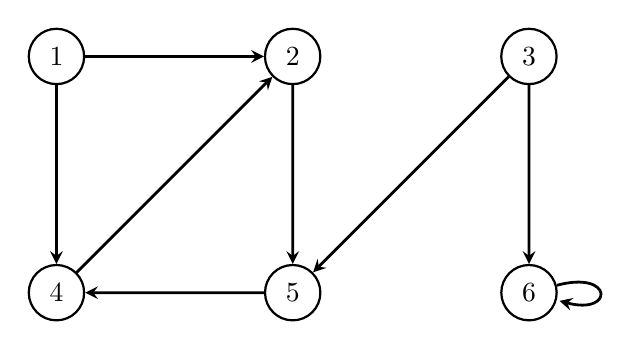
\begin{tikzpicture}[
        scale=1.5,                    % Scale up the entire diagram
        node distance=3cm,            % Increased spacing between nodes
        every node/.style={
            circle, 
            draw, 
            minimum size=2em,       % Slightly larger nodes
            inner sep=4pt             % More internal padding
        },
        >=stealth,
        thick,
        arrow/.style={->, line width=1pt}
    ]
        % 节点
        \node (1) {1};
        \node (4) [below of=1] {4};
        \node (2) [right of=1] {2};
        \node (5) [below of=2] {5};
        \node (3) [right of=2] {3};
        \node (6) [below of=3] {6};
        
        % 边
        \draw[arrow] (1) -- (2);
        \draw[arrow] (1) -- (4);
        \draw[arrow] (4) -- (2);
        \draw[arrow] (2) -- (5);
        \draw[arrow] (5) -- (4);
        \draw[arrow] (3) -- (5);
        \draw[arrow] (3) -- (6);
        \draw[arrow] (6) edge [loop right] (6);
    \end{tikzpicture}
    \caption{图9-1}
    \label{fig:9-1}
\end{figure}

\begin{enumerate}
    \item \textbf{初始化,开始第一轮遍历:}

    \begin{itemize}
        \item 所有节点染白,parent = -,dis = $\infty$
        \item 3入队,dis = 0
    \end{itemize}

    \begin{lstlisting}[style=algorithmPPT]
    BFS-WALKER(G) // BFS遍历器
    foreach v in [1,2,3,4,5,6] do
        v.color:=WHITE; 
        v.parent=NULL 
        v.dis:=+∞;
    foreach v in [3,1,2,4,5,6] do // 从3开始遍历
        if v.color == WHITE then
            BFS(v)
        \end{lstlisting}

    \begin{lstlisting}[style=algorithmPPT]
            BFS(3)
                Initialize an empty queue queNode;
                3.color:=GRAY; // 3 染灰
                3.dis:=0; // 3 dis=0
                queNode.ENQUEUE(3); // 3 入队
        \end{lstlisting}

    \begin{figure}[htbp]
        \begin{minipage}[b]{0.6\textwidth}    % 使用[b]底部对齐,略微减小宽度留间隙
            \centering
            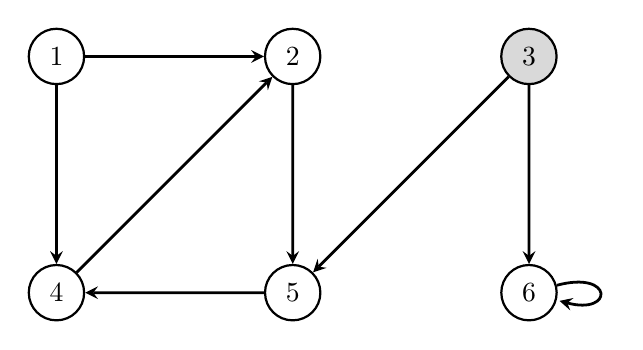
\begin{tikzpicture}[
                scale=1.5,                    % 恢复原始比例
                node distance=3cm,            % 恢复原始间距
                every node/.style={
                    circle, 
                    draw, 
                    minimum size=2em,         % 恢复原始节点大小
                    inner sep=4pt             % 恢复原始内边距
                },
                >=stealth,
                thick,
                arrow/.style={->, line width=1pt}
            ]
                % 节点
                \node (1) {1};
                \node (4) [below of=1] {4};
                \node (2) [right of=1] {2};
                \node (5) [below of=2] {5};
                \node[fill=gray!30] (3) [right of=2] {3};
                \node (6) [below of=3] {6};
                
                % 边
                \draw[arrow] (1) -- (2);
                \draw[arrow] (1) -- (4);
                \draw[arrow] (4) -- (2);
                \draw[arrow] (2) -- (5);
                \draw[arrow] (5) -- (4);
                \draw[arrow] (3) -- (5);
                \draw[arrow] (3) -- (6);
                \draw[arrow] (6) edge [loop right] (6);
            \end{tikzpicture}
            \caption{图9-1-0}
            \label{fig:9-1-0}
        \end{minipage}%
        \hfill%                              % 添加水平填充
        \begin{minipage}[b]{0.4\textwidth}    % 使用[b]底部对齐
            \centering
            \begin{tabular}{|c|c|c|}
                \hline
                节点编号 & Parent & dis值 \\
                \hline
                1 & - & $\infty$ \\
                2 & - & $\infty$ \\
                3 & - & 0 \\
                4 & - & $\infty$ \\
                5 & - & $\infty$ \\
                6 & - & $\infty$ \\
                \hline
            \end{tabular}
            \caption{图9-1-0的BFS结果}
            \label{tab:graph9-1-0-bfs}
        \end{minipage}
    \end{figure}

    \pagebreak

    \item \textbf{第一层(dis = 0):}

    \begin{itemize}
        \item 访问节点3:
        \begin{itemize}
            \item 邻居节点为5和6。
            \item 设置节点5和6的 dis = 1,parent = 3。
            \item 将节点5和6入队。
        \end{itemize}

    \begin{lstlisting}[style=algorithmPPT]
                while queNode = [3] != empty do
                    w:=queNode.DEQUE(); // 队头 3 出队,赋给 w
                    foreach neighbor [5,6] of w = 3 do
                        if 5.color==WHITE then
                            5.color:=GRAY; // 5 染灰
                            5.parent:=3; // 5 parent=3
                            5.dis:=3.dis+1; // 5 dis=1
                            queNode.ENQUEUE(5); // 5 入队
                        if 6.color==WHITE then
                            6.color:=GRAY; // 6 染灰
                            6.parent:=3; // 6 parent=3
                            6.dis:=3.dis+1; // 6 dis=1
                            queNode.ENQUEUE(6); // 6 入队
                    <processing of node w>;
                    3.color:=BLACK; // 3 染黑
                \end{lstlisting}
    \end{itemize}

    \begin{figure}[htbp]
        \begin{minipage}[b]{0.6\textwidth}    % 使用[b]底部对齐,略微减小宽度留间隙
            \centering
            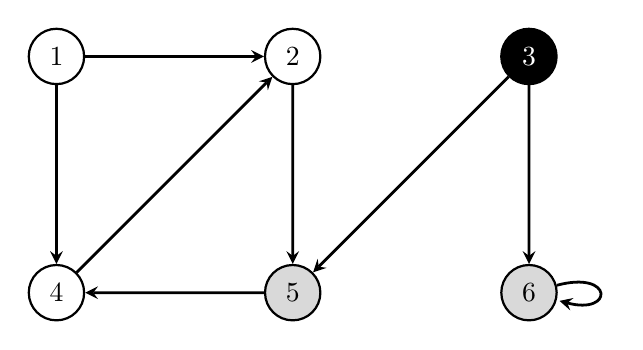
\begin{tikzpicture}[
                scale=1.5,                    % 恢复原始比例
                node distance=3cm,            % 恢复原始间距
                every node/.style={
                    circle, 
                    draw, 
                    minimum size=2em,         % 恢复原始节点大小
                    inner sep=4pt             % 恢复原始内边距
                },
                >=stealth,
                thick,
                arrow/.style={->, line width=1pt}
            ]
                % 节点
                \node (1) {1};
                \node (4) [below of=1] {4};
                \node (2) [right of=1] {2};
                \node[fill=gray!30] (5) [below of=2] {5};  % 灰色节点
                \node[fill=black!100, text=white] (3) [right of=2] {3};  % 黑色节点,白色文字
                \node[fill=gray!30] (6) [below of=3] {6};  % 灰色节点
                
                % 边
                \draw[arrow] (1) -- (2);
                \draw[arrow] (1) -- (4);
                \draw[arrow] (4) -- (2);
                \draw[arrow] (2) -- (5);
                \draw[arrow] (5) -- (4);
                \draw[arrow] (3) -- (5);
                \draw[arrow] (3) -- (6);
                \draw[arrow] (6) edge [loop right] (6);
            \end{tikzpicture}
            \caption{图9-1-1}
            \label{fig:9-1-1}
        \end{minipage}%
        \hfill%                              % 添加水平填充
        \begin{minipage}[b]{0.4\textwidth}    % 使用[b]底部对齐
            \centering
            \begin{tabular}{|c|c|c|}
                \hline
                节点编号 & Parent & dis值 \\
                \hline
                1 & - & $\infty$ \\
                2 & - & $\infty$ \\
                3 & - & 0 \\
                4 & - & $\infty$ \\
                5 & 3 & 1 \\
                6 & 3 & 1 \\
                \hline
            \end{tabular}
            \caption{图9-1-1的BFS结果}
            \label{tab:graph9-1-1-bfs}
        \end{minipage}
    \end{figure}
    
    \pagebreak

    \item \textbf{第二层(dis = 1):}

    \begin{itemize}
        \item 访问节点5:
        \begin{itemize}
            \item 邻居节点为4。
            \item 设置节点4的 dis = 2,parent = 5。
            \item 将节点4入队。
        \end{itemize}
    \end{itemize}

    \begin{lstlisting}[style=algorithmPPT]
                while queNode = [5,6] != empty do // 数字序 5<6
                    w:=queNode.DEQUE(); // 队头 5 出队,赋给 w
                    foreach neighbor [4] of w = 5 do
                        if 4.color==WHITE then
                            4.color:=GRAY; // 4 染灰
                            4.parent:=5; // 4 parent=5
                            4.dis:=5.dis+1; // 4 dis=2
                            queNode.ENQUEUE(4); // 4 入队
                    <processing of node 5>;
                    5.color:=BLACK; // 5 染黑
                \end{lstlisting}    

    \begin{itemize}
        \item 访问节点6:
        \begin{itemize}
            \item 邻居节点为自身,无需操作。
        \end{itemize}
    \end{itemize}


    \begin{lstlisting}[style=algorithmPPT]
                while queNode = [6,4] != empty do
                    w:=queNode.DEQUE(); // 队头 6 出队,赋给 w
                    foreach neighbor [6] of w = 6 do // 6 邻居是自己
                        if 6.color==WHITE then // False 
                    <processing of node 6>;
                    6.color:=BLACK; // 6 染黑        
                \end{lstlisting}  
                
    \begin{figure}[htbp]
        \begin{minipage}[b]{0.6\textwidth}    % 使用[b]底部对齐,略微减小宽度留间隙
            \centering
            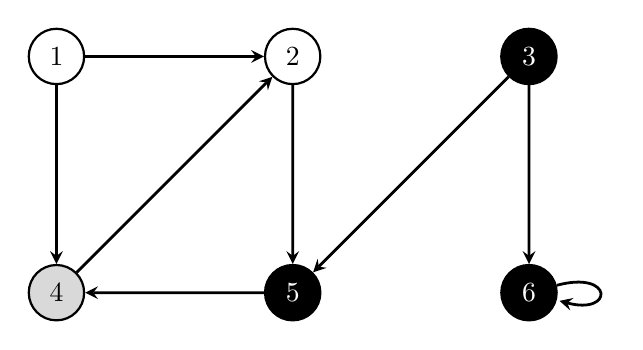
\begin{tikzpicture}[
                scale=1.5,                    % 恢复原始比例
                node distance=3cm,            % 恢复原始间距
                every node/.style={
                    circle, 
                    draw, 
                    minimum size=2em,         % 恢复原始节点大小
                    inner sep=4pt             % 恢复原始内边距
                },
                >=stealth,
                thick,
                arrow/.style={->, line width=1pt}
            ]
                % 节点
                \node (1) {1};
                \node[fill=gray!30] (4) [below of=1] {4};  % 灰色节点
                \node (2) [right of=1] {2};
                \node[fill=black!100, text=white]  (5) [below of=2] {5}; % 黑色节点,白色文字
                \node[fill=black!100, text=white] (3) [right of=2] {3};  % 黑色节点,白色文字
                \node[fill=black!100, text=white]  (6) [below of=3] {6}; % 黑色节点,白色文字
                
                % 边
                \draw[arrow] (1) -- (2);
                \draw[arrow] (1) -- (4);
                \draw[arrow] (4) -- (2);
                \draw[arrow] (2) -- (5);
                \draw[arrow] (5) -- (4);
                \draw[arrow] (3) -- (5);
                \draw[arrow] (3) -- (6);
                \draw[arrow] (6) edge [loop right] (6);
            \end{tikzpicture}
            \caption{图9-1-2}
            \label{fig:9-1-2}
        \end{minipage}%
        \hfill%                              % 添加水平填充
        \begin{minipage}[b]{0.4\textwidth}    % 使用[b]底部对齐
            \centering
            \begin{tabular}{|c|c|c|}
                \hline
                节点编号 & Parent & dis值 \\
                \hline
                1 & - & $\infty$ \\
                2 & - & $\infty$ \\
                3 & - & 0 \\
                4 & 5 & 2 \\
                5 & 3 & 1 \\
                6 & 3 & 1 \\
                \hline
            \end{tabular}
            \caption{图9-1-2的BFS结果}
            \label{tab:graph9-1-2-bfs}
        \end{minipage}
    \end{figure}
            
    \pagebreak

    \item \textbf{第三层(dis = 2):}

    \begin{itemize}
        \item 访问节点4:
        \begin{itemize}
            \item 邻居节点为2。
            \item 设置节点2的 dis = 3,parent = 4。
            \item 将节点2入队。
        \end{itemize}
    \end{itemize}

    \begin{lstlisting}[style=algorithmPPT]
                while queNode = [4] != empty do
                    w:=queNode.DEQUE(); // 队头 4 出队,赋给 w
                    foreach neighbor [2] of w = 4 do 
                        if 2.color==WHITE then
                            2.color:=GRAY; // 2 染灰
                            2.parent:=4; // 2 parent=4
                            2.dis:=4.dis+1; // 2 dis=3
                            queNode.ENQUEUE(2); // 2 入队
                    <processing of node 4>;
                    4.color:=BLACK; // 4 染黑        
                \end{lstlisting}    

    \begin{figure}[htbp]
        \begin{minipage}[b]{0.6\textwidth}    % 使用[b]底部对齐,略微减小宽度留间隙
            \centering
            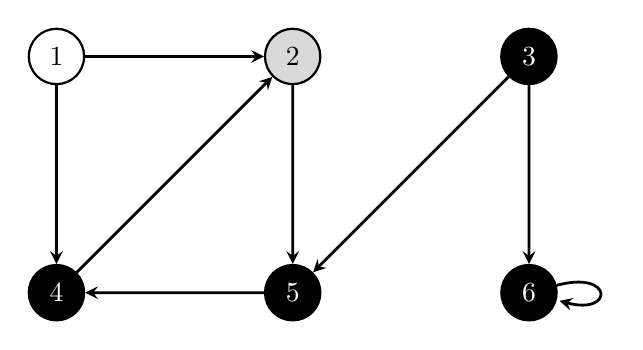
\begin{tikzpicture}[
                scale=1.5,                    % 恢复原始比例
                node distance=3cm,            % 恢复原始间距
                every node/.style={
                    circle, 
                    draw, 
                    minimum size=2em,         % 恢复原始节点大小
                    inner sep=4pt             % 恢复原始内边距
                },
                >=stealth,
                thick,
                arrow/.style={->, line width=1pt}
            ]
                % 节点
                \node (1) {1};
                \node[fill=black!100, text=white] (4) [below of=1] {4};  % 灰色节点
                \node[fill=gray!30] (2) [right of=1] {2};
                \node[fill=black!100, text=white]  (5) [below of=2] {5}; % 黑色节点,白色文字
                \node[fill=black!100, text=white] (3) [right of=2] {3};  % 黑色节点,白色文字
                \node[fill=black!100, text=white]  (6) [below of=3] {6}; % 黑色节点,白色文字
                
                % 边
                \draw[arrow] (1) -- (2);
                \draw[arrow] (1) -- (4);
                \draw[arrow] (4) -- (2);
                \draw[arrow] (2) -- (5);
                \draw[arrow] (5) -- (4);
                \draw[arrow] (3) -- (5);
                \draw[arrow] (3) -- (6);
                \draw[arrow] (6) edge [loop right] (6);
            \end{tikzpicture}
            \caption{图9-1-3}
            \label{fig:9-1-3}
        \end{minipage}%
        \hfill%                              % 添加水平填充
        \begin{minipage}[b]{0.4\textwidth}    % 使用[b]底部对齐
            \centering
            \begin{tabular}{|c|c|c|}
                \hline
                节点编号 & Parent & dis值 \\
                \hline
                1 & - & $\infty$ \\
                2 & 4 & 3 \\
                3 & - & 0 \\
                4 & 5 & 2 \\
                5 & 3 & 1 \\
                6 & 3 & 1 \\
                \hline
            \end{tabular}
            \caption{图9-1-3的BFS结果}
            \label{tab:graph9-1-3-bfs}
        \end{minipage}
    \end{figure}

    \pagebreak

    \item \textbf{第四层(dis = 3):}

    \begin{itemize}
        \item 访问节点2:
        \begin{itemize}
            \item 邻居节点为5,5已出队,无需操作。
        \end{itemize}
    \end{itemize}
    
    \begin{lstlisting}[style=algorithmPPT]
                while queNode = [2] != empty do
                    w:=queNode.DEQUE(); // 队头 2 出队,赋给 w
                    foreach neighbor [5] of w = 2 do 
                        if 5.color==WHITE then // False
                    <processing of node 2>;
                    2.color:=BLACK; // 2 染黑        
        \end{lstlisting}    

    \begin{figure}[htbp]
    \begin{minipage}[b]{0.6\textwidth}    % 使用[b]底部对齐,略微减小宽度留间隙
        \centering
        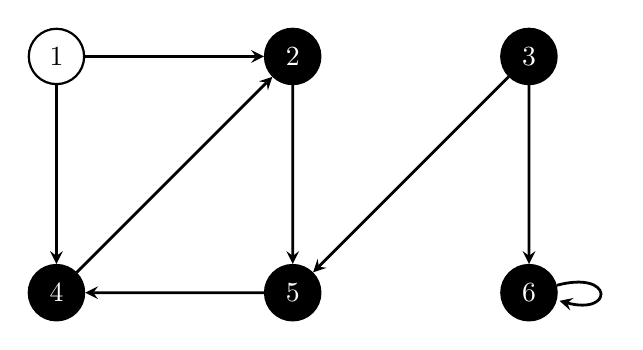
\begin{tikzpicture}[
            scale=1.5,                    % 恢复原始比例
            node distance=3cm,            % 恢复原始间距
            every node/.style={
                circle, 
                draw, 
                minimum size=2em,         % 恢复原始节点大小
                inner sep=4pt             % 恢复原始内边距
            },
            >=stealth,
            thick,
            arrow/.style={->, line width=1pt}
        ]
            % 节点
            \node (1) {1};
            \node[fill=black!100, text=white] (4) [below of=1] {4};  % 灰色节点
            \node[fill=black!100, text=white] (2) [right of=1] {2};
            \node[fill=black!100, text=white]  (5) [below of=2] {5}; % 黑色节点,白色文字
            \node[fill=black!100, text=white] (3) [right of=2] {3};  % 黑色节点,白色文字
            \node[fill=black!100, text=white]  (6) [below of=3] {6}; % 黑色节点,白色文字
            
            % 边
            \draw[arrow] (1) -- (2);
            \draw[arrow] (1) -- (4);
            \draw[arrow] (4) -- (2);
            \draw[arrow] (2) -- (5);
            \draw[arrow] (5) -- (4);
            \draw[arrow] (3) -- (5);
            \draw[arrow] (3) -- (6);
            \draw[arrow] (6) edge [loop right] (6);
        \end{tikzpicture}
        \caption{图9-1-4}
        \label{fig:9-1-4}
    \end{minipage}%
    \hfill%                              % 添加水平填充
    \begin{minipage}[b]{0.4\textwidth}    % 使用[b]底部对齐
        \centering
        \begin{tabular}{|c|c|c|}
            \hline
            节点编号 & Parent & dis值 \\
            \hline
            1 & - & $\infty$ \\
            2 & 4 & 3 \\
            3 & - & 0 \\
            4 & 5 & 2 \\
            5 & 3 & 1 \\
            6 & 3 & 1 \\
            \hline
        \end{tabular}
        \caption{图9-1-4的BFS结果}
        \label{tab:graph9-1-4-bfs}
    \end{minipage}
    \end{figure}
    
    \item \textbf{开始第二轮遍历:}

    \begin{itemize}
        \item 1入队,dis = 0
    \end{itemize}

    \begin{lstlisting}[style=algorithmPPT]
    foreach v in [3,1,2,4,5,6] do // 1为白色
        if v.color == WHITE then
            BFS(v)
        \end{lstlisting}

    \begin{lstlisting}[style=algorithmPPT]
            BFS(1)
                Initialize an empty queue queNode;
                1.color:=GRAY; // 1 染灰
                1.dis:=0; // 1 dis=0
                queNode.ENQUEUE(1); // 1 入队
        \end{lstlisting}

    \begin{figure}[htbp]
        \begin{minipage}[b]{0.6\textwidth}    % 使用[b]底部对齐,略微减小宽度留间隙
            \centering
            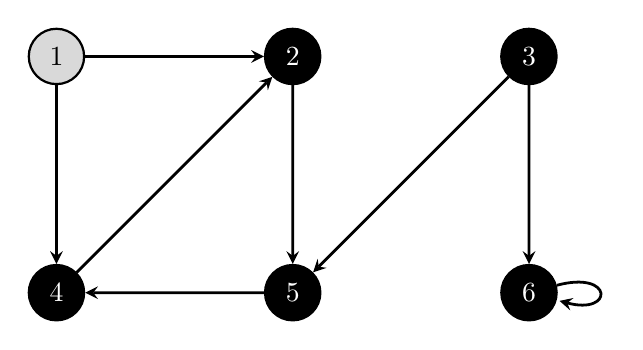
\begin{tikzpicture}[
                scale=1.5,                    % 恢复原始比例
                node distance=3cm,            % 恢复原始间距
                every node/.style={
                    circle, 
                    draw, 
                    minimum size=2em,         % 恢复原始节点大小
                    inner sep=4pt             % 恢复原始内边距
                },
                >=stealth,
                thick,
                arrow/.style={->, line width=1pt}
            ]
                % 节点
                \node[fill=gray!30] (1) {1};
                \node[fill=black!100, text=white] (4) [below of=1] {4};  % 灰色节点
                \node[fill=black!100, text=white] (2) [right of=1] {2};
                \node[fill=black!100, text=white]  (5) [below of=2] {5}; % 黑色节点,白色文字
                \node[fill=black!100, text=white] (3) [right of=2] {3};  % 黑色节点,白色文字
                \node[fill=black!100, text=white]  (6) [below of=3] {6}; % 黑色节点,白色文字
                
                % 边
                \draw[arrow] (1) -- (2);
                \draw[arrow] (1) -- (4);
                \draw[arrow] (4) -- (2);
                \draw[arrow] (2) -- (5);
                \draw[arrow] (5) -- (4);
                \draw[arrow] (3) -- (5);
                \draw[arrow] (3) -- (6);
                \draw[arrow] (6) edge [loop right] (6);
            \end{tikzpicture}
            \caption{图9-1-5}
            \label{fig:9-1-5}
        \end{minipage}%
        \hfill%                              % 添加水平填充
        \begin{minipage}[b]{0.4\textwidth}    % 使用[b]底部对齐
            \centering
            \begin{tabular}{|c|c|c|}
                \hline
                节点编号 & Parent & dis值 \\
                \hline
                1 & - & 0 \\
                2 & 4 & 3 \\
                3 & - & 0 \\
                4 & 5 & 2 \\
                5 & 3 & 1 \\
                6 & 3 & 1 \\
                \hline
            \end{tabular}
            \caption{图9-1-5的BFS结果}
            \label{tab:graph9-1-5-bfs}
        \end{minipage}
    \end{figure}

    \pagebreak

    \item \textbf{第二轮,第一层(dis = 0):}
    
    \begin{itemize}
        \item 访问节点1:
        \begin{itemize}
            \item 邻居节点为2和4。2和4为黑色,无需操作。
        \end{itemize}
    \end{itemize}

    \begin{lstlisting}[style=algorithmPPT]
                while queNode = [1] != empty do
                    w:=queNode.DEQUE(); // 队头 1 出队,赋给 w
                    foreach neighbor [2,4] of w = 1 do
                        if 2.color==WHITE then // 2.color=BLACK False
                        if 4.color==WHITE then // 4.color=BLACK False
                    <processing of node w>;
                    1.color:=BLACK; // 1 染黑
        \end{lstlisting}
 
    \begin{figure}[htbp]
        \begin{minipage}[b]{0.6\textwidth}    % 使用[b]底部对齐,略微减小宽度留间隙
            \centering
            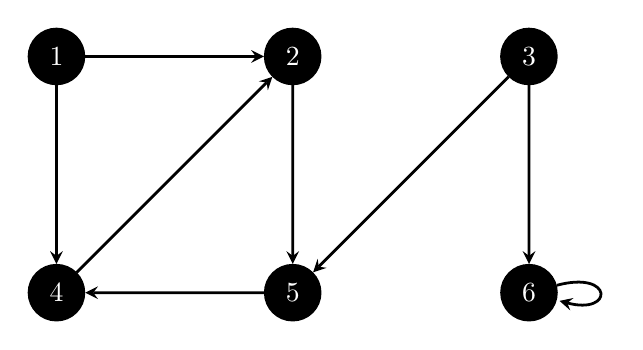
\begin{tikzpicture}[
                scale=1.5,                    % 恢复原始比例
                node distance=3cm,            % 恢复原始间距
                every node/.style={
                    circle, 
                    draw, 
                    minimum size=2em,         % 恢复原始节点大小
                    inner sep=4pt             % 恢复原始内边距
                },
                >=stealth,
                thick,
                arrow/.style={->, line width=1pt}
            ]
                % 节点
                \node[fill=black!100, text=white] (1) {1};
                \node[fill=black!100, text=white] (4) [below of=1] {4};
                \node[fill=black!100, text=white] (2) [right of=1] {2};
                \node[fill=black!100, text=white] (5) [below of=2] {5};  % 灰色节点
                \node[fill=black!100, text=white] (3) [right of=2] {3};  % 黑色节点,白色文字
                \node[fill=black!100, text=white] (6) [below of=3] {6};  % 灰色节点
                
                % 边
                \draw[arrow] (1) -- (2);
                \draw[arrow] (1) -- (4);
                \draw[arrow] (4) -- (2);
                \draw[arrow] (2) -- (5);
                \draw[arrow] (5) -- (4);
                \draw[arrow] (3) -- (5);
                \draw[arrow] (3) -- (6);
                \draw[arrow] (6) edge [loop right] (6);
            \end{tikzpicture}
            \caption{图9-1-6}
            \label{fig:9-1-6}
        \end{minipage}%
        \hfill%                              % 添加水平填充
        \begin{minipage}[b]{0.4\textwidth}    % 使用[b]底部对齐
            \centering
            \begin{tabular}{|c|c|c|}
                \hline
                节点编号 & Parent & dis值 \\
                \hline
                1 & - & 0 \\
                2 & 4 & 3 \\
                3 & - & 0 \\
                4 & 5 & 2 \\
                5 & 3 & 1 \\
                6 & 3 & 1 \\
                \hline
            \end{tabular}
            \caption{图9-1-6的BFS结果}
            \label{tab:graph9-1-6-bfs}
        \end{minipage}
    \end{figure}


    \item \textbf{结束:}

    \begin{itemize}
        \item 队列为空,while循环结束。
        \item 外层节点全黑,BFS结束。
    \end{itemize}

    \begin{lstlisting}[style=algorithmPPT]
                while queNode = [] != empty do   // queNode = [] False
        \end{lstlisting}    

    \begin{lstlisting}[style=algorithmPPT]
    foreach v in [3,1,2,4,5,6] do //全部为黑色
        if v.color == WHITE then
            BFS(v)
        \end{lstlisting}

    \begin{figure}[htbp]
    \begin{minipage}[b]{0.6\textwidth}    % 使用[b]底部对齐,略微减小宽度留间隙
        \centering
        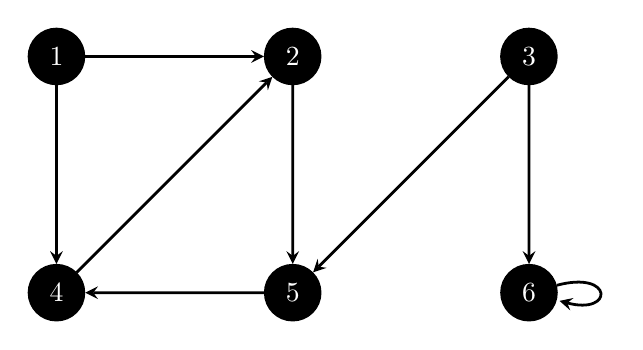
\begin{tikzpicture}[
            scale=1.5,                    % 恢复原始比例
            node distance=3cm,            % 恢复原始间距
            every node/.style={
                circle, 
                draw, 
                minimum size=2em,         % 恢复原始节点大小
                inner sep=4pt             % 恢复原始内边距
            },
            >=stealth,
            thick,
            arrow/.style={->, line width=1pt}
        ]
            % 节点
            \node[fill=black!100, text=white] (1) {1};
            \node[fill=black!100, text=white] (4) [below of=1] {4};  % 灰色节点
            \node[fill=black!100, text=white] (2) [right of=1] {2};
            \node[fill=black!100, text=white]  (5) [below of=2] {5}; % 黑色节点,白色文字
            \node[fill=black!100, text=white] (3) [right of=2] {3};  % 黑色节点,白色文字
            \node[fill=black!100, text=white]  (6) [below of=3] {6}; % 黑色节点,白色文字
            
            % 边
            \draw[arrow] (1) -- (2);
            \draw[arrow] (1) -- (4);
            \draw[arrow] (4) -- (2);
            \draw[arrow] (2) -- (5);
            \draw[arrow] (5) -- (4);
            \draw[arrow] (3) -- (5);
            \draw[arrow] (3) -- (6);
            \draw[arrow] (6) edge [loop right] (6);
        \end{tikzpicture}
        \caption{图9-1-7}
        \label{fig:9-1-7}
    \end{minipage}%
    \hfill%                              % 添加水平填充
    \begin{minipage}[b]{0.4\textwidth}    % 使用[b]底部对齐
        \centering
        \begin{tabular}{|c|c|c|}
            \hline
            节点编号 & Parent & dis值 \\
            \hline
            1 & - & 0 \\
            2 & 4 & 3 \\
            3 & - & 0 \\
            4 & 5 & 2 \\
            5 & 3 & 1 \\
            6 & 3 & 1 \\
            \hline
        \end{tabular}
        \caption{图9-1-7的BFS结果}
        \label{tab:graph9-1-7-bfs}
    \end{minipage}
    \end{figure}
    
\end{enumerate}

\clearpage 

\subsubsection{对图9-2执行BFS并确定每个节点的parent和dis值}

\begin{figure}[htbp]
    \centering
    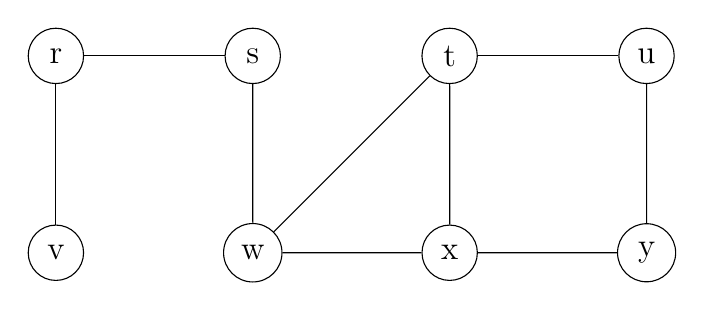
\begin{tikzpicture}[
        scale=1.5,
        node distance=2.5cm,
        every node/.style={
            circle, 
            draw, 
            minimum size=2em,
            inner sep=4pt,
            font=\large
        }
    ]
        % First component (r-s-v-w)
        \node (r) {r};
        \node (s) [right of=r] {s};
        \node (v) [below of=r] {v};
        \node (w) [below of=s] {w};
        
        % Second component (t-u-x-y)
        \node (t) [right of=s] {t};
        \node (u) [right of=t] {u};
        \node (x) [below of=t] {x};
        \node (y) [below of=u] {y};
        
        % Edges
        \draw (r) -- (s);
        \draw (r) -- (v);
        \draw (s) -- (w);
        \draw (t) -- (u);
        \draw (t) -- (x);
        \draw (u) -- (y);
        \draw (x) -- (y);
        \draw (w) -- (t);
        \draw (w) -- (x);
    \end{tikzpicture}
    \caption{图9-2}
    \label{fig:9-2}
\end{figure}

\begin{enumerate}

    \item \textbf{初始化:}

    \begin{itemize}
        \item 所有节点染白,parent = -,dis = $\infty$
        \item u入队,dis = 0
    \end{itemize}

    \begin{lstlisting}[style=algorithmPPT]
        BFS-WARRER(G)
        foreach node v in [r,x,t,u,v,w,x,y] do
            v.color:=WHITE; 
            v.parent=NULL 
            v.dis:=+∞;
        foreach node v in [u,r,x,t,v,w,x,y] do
            if v.color == WHITE then
                BFS(v)
                BFS(u)
                    Initialize an empty queue queNode;
                    u.color:=GRAY; // u 染灰
                    u.dis:=0; // u dis=0
                    queNode.ENQUEUE(u); // u 入队
                \end{lstlisting}

    \begin{figure}[htbp]
        \begin{minipage}[b]{0.6\textwidth}    % 使用[b]底部对齐,略微减小宽度留间隙
            \centering
                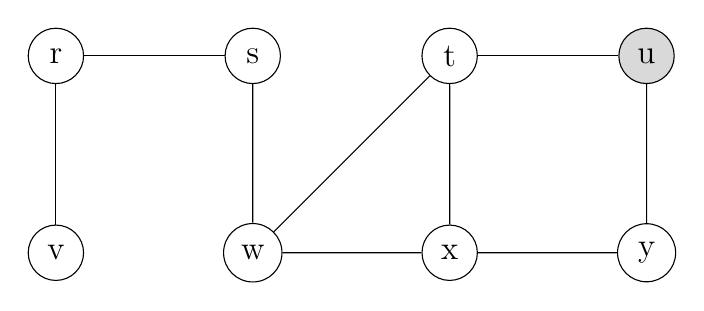
\begin{tikzpicture}[
                    scale=1.5,
                    node distance=2.5cm,
                    every node/.style={
                        circle, 
                        draw, 
                        minimum size=2em,
                        inner sep=4pt,
                        font=\large
                    }
                ]
                    \node (r) {r};
                    \node (s) [right of=r] {s};
                    \node (t) [right of=s] {t};
                    \node[fill=gray!30] (u) [right of=t] {u};
                    \node (v) [below of=r] {v};
                    \node (w) [below of=s] {w};
                    \node (x) [below of=t] {x};
                    \node (y) [below of=u] {y};
                    
                    % Edges
                    \draw (r) -- (s);
                    \draw (r) -- (v);
                    \draw (s) -- (w);
                    \draw (t) -- (u);
                    \draw (t) -- (x);
                    \draw (u) -- (y);
                    \draw (x) -- (y);
                    \draw (w) -- (t);
                    \draw (w) -- (x);
                \end{tikzpicture}
                \caption{图9-2-0}
                \label{fig:9-2-0}
        \end{minipage}%
        \hfill%                              % 添加水平填充
        \begin{minipage}[b]{0.4\textwidth}    % 使用[b]底部对齐
            \centering
                \begin{tabular}{|c|c|c|}
                    \hline
                    节点 & Parent & dis值 \\
                    \hline
                    r & - & $\infty$ \\
                    s & - & $\infty$ \\
                    t & - & $\infty$ \\
                    u & - & 0 \\
                    v & - & $\infty$ \\
                    w & - & $\infty$ \\
                    x & - & $\infty$ \\
                    y & - & $\infty$ \\
                    \hline
                \end{tabular}
                \caption{图9-2-0的BFS结果}
                \label{tab:graph9-2-0-bfs}
        \end{minipage}
    \end{figure}
    
    \pagebreak
    
    \item \textbf{第一层(dis = 0):}
    
    \begin{itemize}
        \item 访问节点u,发现邻居t和y
        \item 设置t和y的dis值为1,parent为u

        \begin{lstlisting}[style=algorithmPPT]
                while queNode = [u] != empty do
                    w1:=queNode.DEQUEUE(); // 队头 u 出队,赋给 w1
                    foreach neighbor [t,y] of w1 = u do
                        if t.color==WHITE then
                            t.color:=GRAY; // t 染灰
                            t.parent:=u; // t parent=u
                            t.dis:=u.dis+1; // t dis=1
                            queNode.ENQUEUE(t); // t 入队
                        if y.color==WHITE then
                            y.color:=GRAY; // y 染灰
                            y.parent:=u; // y parent=u
                            y.dis:=u.dis+1; // y dis=1
                            queNode.ENQUEUE(y); // y 入队
                    <processing of node u>;
                    u.color:=BLACK; // u 染黑
                \end{lstlisting}
    \end{itemize}

    \begin{figure}[htbp]
        \begin{minipage}[b]{0.6\textwidth}    % 使用[b]底部对齐,略微减小宽度留间隙
            \centering
                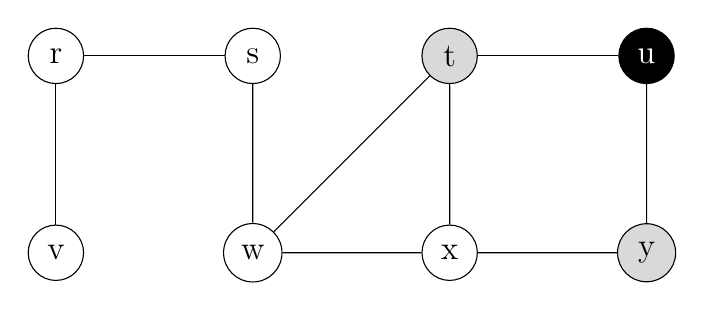
\begin{tikzpicture}[
                    scale=1.5,
                    node distance=2.5cm,
                    every node/.style={
                        circle, 
                        draw, 
                        minimum size=2em,
                        inner sep=4pt,
                        font=\large
                    }
                ]
                    
                    \node (r) {r};
                    \node (s) [right of=r] {s};
                    \node[fill=gray!30] (t) [right of=s] {t};
                    \node[fill=black!100, text=white] (u) [right of=t] {u};
                    \node (v) [below of=r] {v};
                    \node (w) [below of=s] {w};
                    \node (x) [below of=t] {x};
                    \node[fill=gray!30] (y) [below of=u] {y};
                    
                    % Edges
                    \draw (r) -- (s);
                    \draw (r) -- (v);
                    \draw (s) -- (w);
                    \draw (t) -- (u);
                    \draw (t) -- (x);
                    \draw (u) -- (y);
                    \draw (x) -- (y);
                    \draw (w) -- (t);
                    \draw (w) -- (x);
                \end{tikzpicture}
                \caption{图9-2-1}
                \label{fig:9-2-1}
        \end{minipage}%
        \hfill%                              % 添加水平填充
        \begin{minipage}[b]{0.4\textwidth}    % 使用[b]底部对齐
            \centering
                \begin{tabular}{|c|c|c|}
                    \hline
                    节点 & Parent & dis值 \\
                    \hline
                    r & - & $\infty$ \\
                    s & - & $\infty$ \\
                    t & u & 1 \\
                    u & - & 0 \\
                    v & - & $\infty$ \\
                    w & - & $\infty$ \\
                    x & - & $\infty$ \\
                    y & u & 1 \\
                    \hline
                \end{tabular}
            \caption{图9-2-1的BFS结果}
            \label{tab:graph9-2-1-bfs}
        \end{minipage}
    \end{figure}
    
    \pagebreak

    \item \textbf{第二层(dis = 1):}

    \begin{itemize}
        \item 访问t:发现w和x,设置它们的dis值为2,parent为t
    
    \end{itemize}

    \begin{lstlisting}[style=algorithmPPT]
                while queNode = [t,y] != empty do 
                    w1:=queNode.DEQUE(); // 队头 t 出队,赋给 w1
                    foreach neighbor [u,w,x] of w1 = t do
                        if u.color==WHITE then// u.color=BLACK False
                        if w.color==WHITE then
                            w.color:=GRAY; // w 染灰
                            w.parent:=t; // w parent=t
                            w.dis:=t.dis+1; // w dis=2
                            queNode.ENQUEUE(w); // w 入队
                        if x.color==WHITE then
                            x.color:=GRAY; // x 染灰
                            x.parent:=t; // x parent=t
                            x.dis:=t.dis+1; // x dis=2
                            queNode.ENQUEUE(x); // x 入队
                    <processing of node t>;
                    t.color:=BLACK; // t 染黑
                \end{lstlisting}    
        
    \begin{itemize}
        \item 访问y:邻居均已访问或在队列中
    \end{itemize}


    \begin{lstlisting}[style=algorithmPPT]
                while queNode = [y,w,x] != empty do
                    w1:=queNode.DEQUE(); // 队头 y 出队,赋给 w1
                    foreach neighbor [u,x] of w1 = y do 
                        if u.color==WHITE then // u.color=BLACK False
                        if x.color==WHITE then // x.color=GRAY False
                    <processing of node y>;
                    y.color:=BLACK; // y 染黑        
                \end{lstlisting}  
    
    \begin{figure}[htbp]
        \begin{minipage}[b]{0.6\textwidth}    % 使用[b]底部对齐,略微减小宽度留间隙
            \centering
                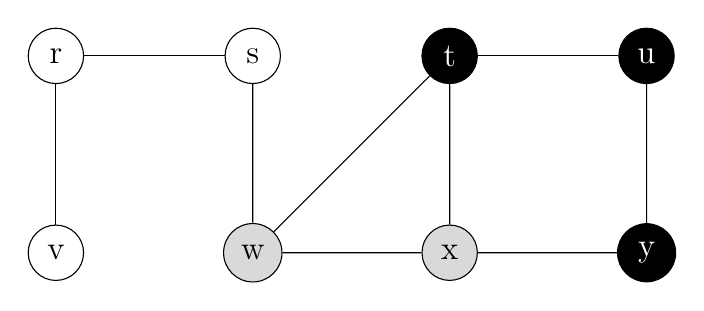
\begin{tikzpicture}[
                    scale=1.5,
                    node distance=2.5cm,
                    every node/.style={
                        circle, 
                        draw, 
                        minimum size=2em,
                        inner sep=4pt,
                        font=\large
                    }
                ]
                    
                    \node (r) {r};
                    \node (s) [right of=r] {s};
                    \node[fill=black!100, text=white] (t) [right of=s] {t};
                    \node[fill=black!100, text=white] (u) [right of=t] {u};
                    \node (v) [below of=r] {v};
                    \node[fill=gray!30] (w) [below of=s] {w};
                    \node[fill=gray!30] (x) [below of=t] {x};
                    \node[fill=black!100, text=white] (y) [below of=u] {y};
                    
                    % Edges
                    \draw (r) -- (s);
                    \draw (r) -- (v);
                    \draw (s) -- (w);
                    \draw (t) -- (u);
                    \draw (t) -- (x);
                    \draw (u) -- (y);
                    \draw (x) -- (y);
                    \draw (w) -- (t);
                    \draw (w) -- (x);
                \end{tikzpicture}
                \caption{图9-2-1}
                \label{fig:9-2-1}
    \end{minipage}%
    \hfill%                              % 添加水平填充
    \begin{minipage}[b]{0.4\textwidth}    % 使用[b]底部对齐
        \centering
            \begin{tabular}{|c|c|c|}
                \hline
                节点 & Parent & dis值 \\
                \hline
                r & - & $\infty$ \\
                s & - & $\infty$ \\
                t & u & 1 \\
                u & - & 0 \\
                v & - & $\infty$ \\
                w & t & 2 \\
                x & t & 2 \\
                y & u & 1 \\
                \hline
            \end{tabular}
        \caption{图9-2-1的BFS结果}
        \label{tab:graph9-2-1-bfs}
    \end{minipage}
    \end{figure}

    \pagebreak 

    \item \textbf{第三层(dis = 2):}
    
    \begin{itemize}
        \item 访问w:发现s,设置其dis值为3,parent为w
    \end{itemize}

    \begin{lstlisting}[style=algorithmPPT]
                while queNode = [w,x] != empty do
                    w1:=queNode.DEQUE(); // 队头 w 出队,赋给 w1
                    foreach neighbor [s,t,x] of w1 = w do
                        if s.color==WHITE then
                            s.color:=GRAY; // s 染灰
                            s.parent:=t; // s parent=w
                            s.dis:=t.dis+1; // s dis=2
                            queNode.ENQUEUE(s); // s 入队
                        if t.color==WHITE then // t.color=BLACK False
                        if x.color==WHITE then// x.color=GRAY False
                    <processing of node w>;
                    w.color:=BLACK; // w 染黑
                \end{lstlisting}    
    
    \begin{itemize}
        \item 访问x:邻居均已访问
    \end{itemize}

    \begin{lstlisting}[style=algorithmPPT]
                while queNode = [x,s] != empty do
                    w1:=queNode.DEQUE(); // 队头 x 出队,赋给 w1
                    foreach neighbor [t,w,y] of w1 = x do 
                        if t.color==WHITE then // t.color=BLACK False
                        if w.color==WHITE then // w.color=BLACK False
                        if y.color==WHITE then // y.color=BLACK False
                    <processing of node x>;
                    x.color:=BLACK; // x 染黑        
                \end{lstlisting}  

    \begin{figure}[htbp]
        \begin{minipage}[b]{0.6\textwidth}    % 使用[b]底部对齐,略微减小宽度留间隙
            \centering
                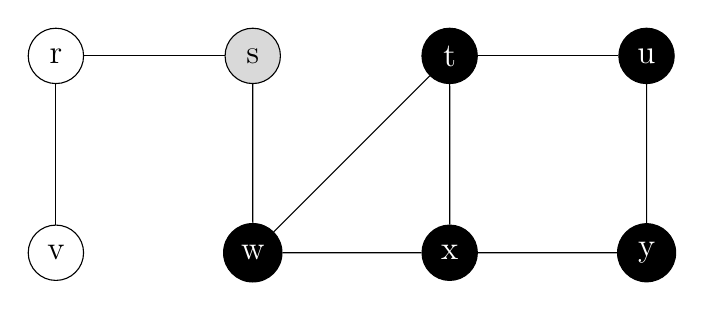
\begin{tikzpicture}[
                    scale=1.5,
                    node distance=2.5cm,
                    every node/.style={
                        circle, 
                        draw, 
                        minimum size=2em,
                        inner sep=4pt,
                        font=\large
                    }
                ]
                    
                    \node (r) {r};
                    \node[fill=gray!30] (s) [right of=r] {s};
                    \node[fill=black!100, text=white] (t) [right of=s] {t};
                    \node[fill=black!100, text=white] (u) [right of=t] {u};
                    \node (v) [below of=r] {v};
                    \node[fill=black!100, text=white] (w) [below of=s] {w};
                    \node[fill=black!100, text=white] (x) [below of=t] {x};
                    \node[fill=black!100, text=white] (y) [below of=u] {y};
                    
                    % Edges
                    \draw (r) -- (s);
                    \draw (r) -- (v);
                    \draw (s) -- (w);
                    \draw (t) -- (u);
                    \draw (t) -- (x);
                    \draw (u) -- (y);
                    \draw (x) -- (y);
                    \draw (w) -- (t);
                    \draw (w) -- (x);
                \end{tikzpicture}
                \caption{图9-2-3}
                \label{fig:9-2-3}
        \end{minipage}%
        \hfill%                              % 添加水平填充
        \begin{minipage}[b]{0.4\textwidth}    % 使用[b]底部对齐
            \centering
                \begin{tabular}{|c|c|c|}
                    \hline
                    节点 & Parent & dis值 \\
                    \hline
                    r & - & $\infty$ \\
                    s & w & 3 \\
                    t & u & 1 \\
                    u & - & 0 \\
                    v & - & $\infty$ \\
                    w & t & 2 \\
                    x & t & 2 \\
                    y & u & 1 \\
                    \hline
                \end{tabular}
                \caption{图9-2-3的BFS结果}
                \label{tab:graph9-2-3-bfs}
        \end{minipage}
    \end{figure}

    \pagebreak

    \item \textbf{第四层(dis = 3):}
    
    \begin{itemize}
        \item 访问s:发现r,设置其dis值为4,parent为s
    \end{itemize}

    \begin{lstlisting}[style=algorithmPPT]
                while queNode = [s] != empty do 
                    w1:=queNode.DEQUE(); // 队头 s 出队,赋给 w1
                    foreach neighbor [r,w] of w1 = s do
                        if r.color==WHITE then
                            r.color:=GRAY; // r 染灰
                            r.parent:=s; // r parent=s
                            r.dis:=s.dis+1; // r dis=4
                            queNode.ENQUEUE(r); // r 入队
                        if w.color==WHITE then // w.color=BLACK False
                    <processing of node s>;
                    s.color:=BLACK; // s 染黑
                \end{lstlisting}    

    \begin{figure}[htbp]
        \begin{minipage}[b]{0.6\textwidth}    % 使用[b]底部对齐,略微减小宽度留间隙
            \centering
                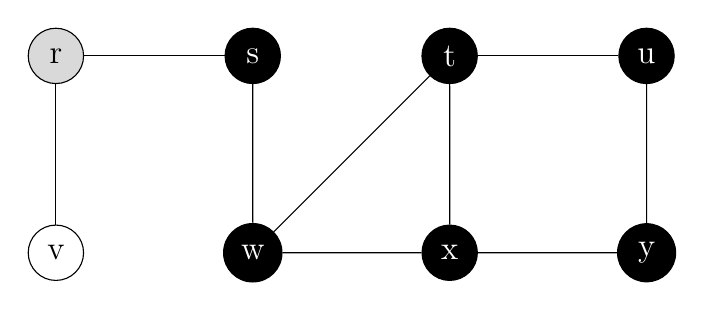
\begin{tikzpicture}[
                    scale=1.5,
                    node distance=2.5cm,
                    every node/.style={
                        circle, 
                        draw, 
                        minimum size=2em,
                        inner sep=4pt,
                        font=\large
                    }
                ]
                    
                    \node[fill=gray!30] (r) {r};
                    \node[fill=black!100, text=white] (s) [right of=r] {s};
                    \node[fill=black!100, text=white] (t) [right of=s] {t};
                    \node[fill=black!100, text=white] (u) [right of=t] {u};
                    \node (v) [below of=r] {v};
                    \node[fill=black!100, text=white] (w) [below of=s] {w};
                    \node[fill=black!100, text=white] (x) [below of=t] {x};
                    \node[fill=black!100, text=white] (y) [below of=u] {y};
                    
                    % Edges
                    \draw (r) -- (s);
                    \draw (r) -- (v);
                    \draw (s) -- (w);
                    \draw (t) -- (u);
                    \draw (t) -- (x);
                    \draw (u) -- (y);
                    \draw (x) -- (y);
                    \draw (w) -- (t);
                    \draw (w) -- (x);
                \end{tikzpicture}
                \caption{图9-2-4}
                \label{fig:9-2-4}
        \end{minipage}%
        \hfill%                              % 添加水平填充
        \begin{minipage}[b]{0.4\textwidth}    % 使用[b]底部对齐
            \centering
                \begin{tabular}{|c|c|c|}
                    \hline
                    节点 & Parent & dis值 \\
                    \hline
                    r & s & 4 \\
                    s & w & 3 \\
                    t & u & 1 \\
                    u & - & 0 \\
                    v & r & 5 \\
                    w & t & 2 \\
                    x & t & 2 \\
                    y & u & 1 \\
                    \hline
                \end{tabular}
                \caption{图9-2-4的BFS结果}
                \label{tab:graph9-2-4-bfs}
        \end{minipage}
    \end{figure}
    
    \pagebreak 

    \item \textbf{第五层(dis = 4):}
    
    \begin{itemize}
        \item 访问r:发现v,设置其dis值为5,parent为r
    \end{itemize}

    \begin{lstlisting}[style=algorithmPPT]
                while queNode = [r] != empty do 
                    w1:=queNode.DEQUE(); // 队头 r 出队,赋给 w1
                    foreach neighbor [s,v] of w1 = r do
                        if s.color==WHITE then // s.color=BLACK False
                        if v.color==WHITE then 
                            v.color:=GRAY; // v 染灰
                            v.parent:=r; // v parent=r
                            v.dis:=r.dis+1; // v dis=5
                            queNode.ENQUEUE(v); // v 入队
                    <processing of node r>;
                    r.color:=BLACK; // r 染黑
        \end{lstlisting}    

    \begin{figure}[htbp]
        \begin{minipage}[b]{0.6\textwidth}    % 使用[b]底部对齐,略微减小宽度留间隙
            \centering
                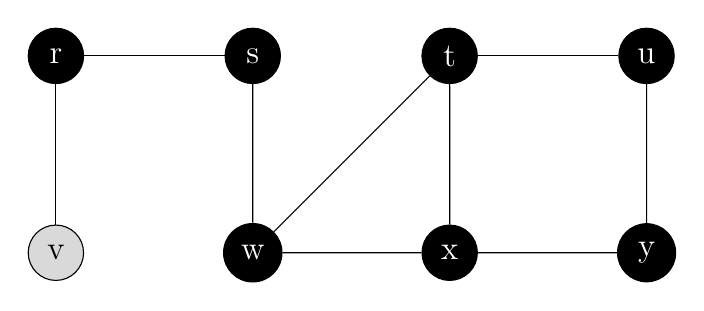
\begin{tikzpicture}[
                    scale=1.5,
                    node distance=2.5cm,
                    every node/.style={
                        circle, 
                        draw, 
                        minimum size=2em,
                        inner sep=4pt,
                        font=\large
                    }
                ]
                    
                    \node[fill=black!100, text=white] (r) {r};
                    \node[fill=black!100, text=white] (s) [right of=r] {s};
                    \node[fill=black!100, text=white] (t) [right of=s] {t};
                    \node[fill=black!100, text=white] (u) [right of=t] {u};
                    \node[fill=gray!30] (v) [below of=r] {v};
                    \node[fill=black!100, text=white] (w) [below of=s] {w};
                    \node[fill=black!100, text=white] (x) [below of=t] {x};
                    \node[fill=black!100, text=white] (y) [below of=u] {y};
                    
                    % Edges
                    \draw (r) -- (s);
                    \draw (r) -- (v);
                    \draw (s) -- (w);
                    \draw (t) -- (u);
                    \draw (t) -- (x);
                    \draw (u) -- (y);
                    \draw (x) -- (y);
                    \draw (w) -- (t);
                    \draw (w) -- (x);
                \end{tikzpicture}
                \caption{图9-2-5}
                \label{fig:9-2-5}
        \end{minipage}%
        \hfill%                              % 添加水平填充
        \begin{minipage}[b]{0.4\textwidth}    % 使用[b]底部对齐
            \centering
            \begin{tabular}{|c|c|c|}
                    \hline
                    节点 & Parent & dis值 \\
                    \hline
                    r & s & 4 \\
                    s & w & 3 \\
                    t & u & 1 \\
                    u & - & 0 \\
                    v & r & 5 \\
                    w & t & 2 \\
                    x & t & 2 \\
                    y & u & 1 \\
                    \hline
                \end{tabular}
                \caption{图9-2-5的BFS结果}
                \label{tab:graph9-2-5-bfs}
        \end{minipage}
    \end{figure}

    \pagebreak
    
    \item \textbf{第六层(dis = 5):}
    
    \begin{itemize}
        \item 访问v:邻居均已访问
    \end{itemize}

    \begin{lstlisting}[style=algorithmPPT]
                while queNode = [v] != empty do 
                    w1:=queNode.DEQUE(); // 队头 v 出队,赋给 w1
                    foreach neighbor [r] of w1 = v do
                        if r.color==WHITE then // r.color=BLACK False
                    <processing of node v>;
                    v.color:=BLACK; // v 染黑
        \end{lstlisting}    

    \begin{figure}[htbp]
        \begin{minipage}[b]{0.6\textwidth}    % 使用[b]底部对齐,略微减小宽度留间隙
            \centering
                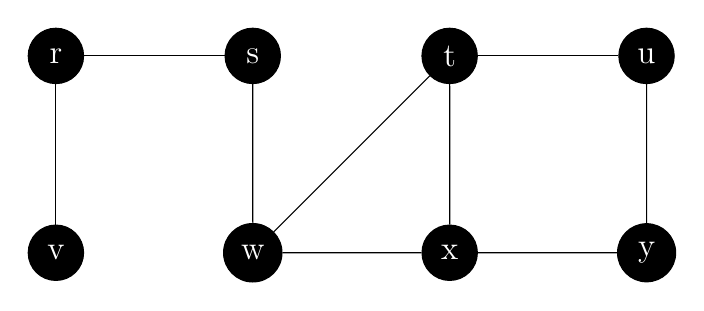
\begin{tikzpicture}[
                    scale=1.5,
                    node distance=2.5cm,
                    every node/.style={
                        circle, 
                        draw, 
                        minimum size=2em,
                        inner sep=4pt,
                        font=\large
                    }
                ]
                    
                    \node[fill=black!100, text=white] (r) {r};
                    \node[fill=black!100, text=white] (s) [right of=r] {s};
                    \node[fill=black!100, text=white] (t) [right of=s] {t};
                    \node[fill=black!100, text=white] (u) [right of=t] {u};
                    \node[fill=black!100, text=white] (v) [below of=r] {v};
                    \node[fill=black!100, text=white] (w) [below of=s] {w};
                    \node[fill=black!100, text=white] (x) [below of=t] {x};
                    \node[fill=black!100, text=white] (y) [below of=u] {y};
                    
                    % Edges
                    \draw (r) -- (s);
                    \draw (r) -- (v);
                    \draw (s) -- (w);
                    \draw (t) -- (u);
                    \draw (t) -- (x);
                    \draw (u) -- (y);
                    \draw (x) -- (y);
                    \draw (w) -- (t);
                    \draw (w) -- (x);
                \end{tikzpicture}
                \caption{图9-2-6}
                \label{fig:9-2-6}
    \end{minipage}%
    \hfill%                              % 添加水平填充
    \begin{minipage}[b]{0.4\textwidth}    % 使用[b]底部对齐
        \centering
        \begin{tabular}{|c|c|c|}
                \hline
                节点 & Parent & dis值 \\
                \hline
                r & s & 4 \\
                s & w & 3 \\
                t & u & 1 \\
                u & - & 0 \\
                v & r & 5 \\
                w & t & 2 \\
                x & t & 2 \\
                y & u & 1 \\
                \hline
            \end{tabular}
            \caption{图9-2-6的BFS结果}
            \label{tab:graph9-2-6-bfs}
    \end{minipage}
    \end{figure}

    \item \textbf{结束}

    \begin{itemize}
        \item 队列为空,while循环结束。
        \item 外层节点全黑,BFS结束。
    \end{itemize}

    \begin{lstlisting}[style=algorithmPPT]
                while queNode = [] != empty do   // queNode = [] False
        \end{lstlisting}    

    \begin{lstlisting}[style=algorithmPPT]
    foreach v in [u,r,s,t,v,w,x,y] do //全部为黑色
        if v.color == WHITE then
            BFS(v)
        \end{lstlisting}

    \begin{figure}[htbp]
        \begin{minipage}[b]{0.6\textwidth}    % 使用[b]底部对齐,略微减小宽度留间隙
            \centering
                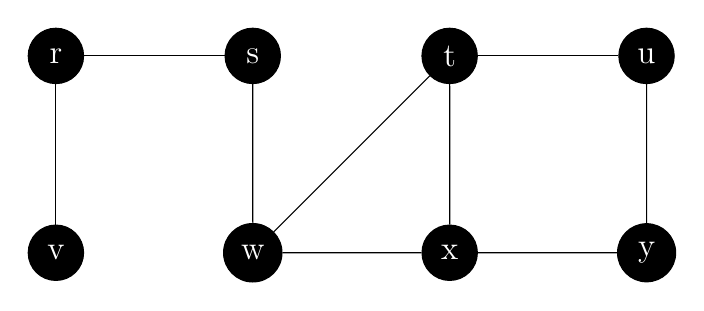
\begin{tikzpicture}[
                    scale=1.5,
                    node distance=2.5cm,
                    every node/.style={
                        circle, 
                        draw, 
                        minimum size=2em,
                        inner sep=4pt,
                        font=\large
                    }
                ]
                    
                    \node[fill=black!100, text=white] (r) {r};
                    \node[fill=black!100, text=white] (s) [right of=r] {s};
                    \node[fill=black!100, text=white] (t) [right of=s] {t};
                    \node[fill=black!100, text=white] (u) [right of=t] {u};
                    \node[fill=black!100, text=white] (v) [below of=r] {v};
                    \node[fill=black!100, text=white] (w) [below of=s] {w};
                    \node[fill=black!100, text=white] (x) [below of=t] {x};
                    \node[fill=black!100, text=white] (y) [below of=u] {y};
                    
                    % Edges
                    \draw (r) -- (s);
                    \draw (r) -- (v);
                    \draw (s) -- (w);
                    \draw (t) -- (u);
                    \draw (t) -- (x);
                    \draw (u) -- (y);
                    \draw (x) -- (y);
                    \draw (w) -- (t);
                    \draw (w) -- (x);
                \end{tikzpicture}
                \caption{图9-2-7}
                \label{fig:9-2-7}
        \end{minipage}%
        \hfill%                              % 添加水平填充
        \begin{minipage}[b]{0.4\textwidth}    % 使用[b]底部对齐
            \centering
            \begin{tabular}{|c|c|c|}
                    \hline
                    节点 & Parent & dis值 \\
                    \hline
                    r & s & 4 \\
                    s & w & 3 \\
                    t & u & 1 \\
                    u & - & 0 \\
                    v & r & 5 \\
                    w & t & 2 \\
                    x & t & 2 \\
                    y & u & 1 \\
                    \hline
                \end{tabular}
                \caption{图9-2-7的BFS结果}
                \label{tab:graph9-2-7-bfs}
        \end{minipage}
    \end{figure}
\end{enumerate}


\pagebreak

\section{有环图的检测}
\subsection{问题描述}

在PPT给出的DFS和BFS框架中,如何解决检测一个图是否存在环的问题?


\subsection{解答}

\pagebreak

\subsubsection{PPT给出的DFS和BFS框架}

\paragraph{1.DFS}

\begin{lstlisting}[style=algorithmPPT]
    DFS(v)
        v.color:=GRAY
        <Preorder processing of node v>
        foreach neighbor w of v do
            if w.color = WHITE then
                <Exploratory processing of edge vw>
                DFS(w)
                <Backtrack processing of edge vw>
            else
                <Checking edge vw>
        <Postorder processing of node v>
        v.color:=BLACK
    \end{lstlisting}

\paragraph{2.BFS}

\begin{lstlisting}[style=algorithmPPT]
    BFS-WARRER(G)  // 应为 BFS-WALKER 广度优先搜索遍历器
    foreach node v in G do
        v.color:=WHITE; 
        v.parent=NULL 
        v.dis:=+∞;
    foreach node v in G do
        if v.color == WHITE then
            BFS(v)
\end{lstlisting}

\begin{lstlisting}[style=algorithmPPT]
            BFS(G)
                Initialize an empty queue queNode;
                v.color:=GRAY;
                v.dis:=0;
                queNode.EUQUE(); // 应为 ENQUEUE 同13行
                while queNode != empty do
                    w:=queNode.DEQUE();
                    foreach neighbor x of w do
                        if x.color==WHITE then
                            x.color:=GRAY;
                            x.parent:=w;
                            x.dis:=w.dis+1;
                            queNode.ENQUEUE(x);
                    <processing of node w>; //我之前的缩进错了
                    w.color:=BLACK;
\end{lstlisting}

\pagebreak

\subsubsection{框架中检测环的方法}

\paragraph{1.DFS\\}

\textbf{适用有向图,无向图:\\}

\begin{lstlisting}[style=algorithm]
    DFS_WALKER(G) // DFS遍历器
    foreach v in G do
        v.color := WHITE
    foreach v in G do
        if v.color == WHITE then
            DFS(v)
\end{lstlisting}

\begin{lstlisting}[style=algorithmPPT]
            DFS(v)
                v.color:=GRAY
                <Preorder processing of node v>
                foreach neighbor w of v do
                    if w.color = WHITE then
                        <Exploratory processing of edge vw>
                        DFS(w)
                        <Backtrack processing of edge vw>              
                    else
                        <Checking edge vw>
                \end{lstlisting}  

\begin{lstlisting}[style=algorithm]
                        if w.color == GRAY then
                            // 发现后向边,存在环
                            return true
                        \end{lstlisting}

\begin{lstlisting}[style=algorithmPPT]
                <Postorder processing of node v>
                v.color:=BLACK
            \end{lstlisting}


\pagebreak

\paragraph{2.BFS\\}

\begin{enumerate}
    \item \textbf{有向图:\\}

    \begin{lstlisting}[style=algorithmPPT]
    BFS-WALKER(G) // BFS遍历器
    foreach node v in G do
        v.color:=WHITE; 
        v.parent=NULL 
        v.dis:=+∞;
    foreach node v in G do
        if v.color == WHITE then
            BFS(v)
        \end{lstlisting}

    \begin{lstlisting}[style=algorithmPPT]
            BFS(G)
                Initialize an empty queue queNode;
                v.color:=GRAY;
                v.dis:=0;
                queNode.ENQUEUE(v);
                while queNode != empty do
                    w:=queNode.DEQUE();
                    foreach neighbor x of w do
                        if x.color==WHITE then
                            x.color:=GRAY;
                            x.parent:=w;
                            x.dis:=w.dis+1;
                            queNode.ENQUEUE(x);
                        
                    \end{lstlisting}

    \begin{lstlisting}[style=algorithm]
                        else if x.color == BLACK then 
                            // 可能是另一棵树的黑色节点
                            // 获取并比较两个节点的所有祖先
                            if hasCommonAncestor(x, w) then
                                // 发现环
                        \end{lstlisting}

    \begin{lstlisting}[style=algorithmPPT]
                    <processing of node w>;
                    w.color:=BLACK;
    \end{lstlisting}

    \begin{lstlisting}[style=algorithm]
    hasCommonAncestor(node1, node2)
        ancestors := new Set()
        cur := node1
        while cur.parent != NULL do
            ancestors.add(cur.parent)
            cur := cur.parent
        
        cur := node2
        while cur.parent != NULL do
            if cur.parent in ancestors then
                return true
            cur := cur.parent
        
        return false
    \end{lstlisting}


    \item \textbf{无向图:\\}

    \begin{lstlisting}[style=algorithmPPT]
    BFS-WALKER(G) // BFS遍历器
        foreach node v in G do
        v.color:=WHITE; 
        v.parent=NULL 
        v.dis:=+∞;
    foreach node v in G do
        if v.color == WHITE then
            BFS(v)
    \end{lstlisting}

    \begin{lstlisting}[style=algorithmPPT]
            BFS(G)
                Initialize an empty queue queNode;
                v.color:=GRAY;
                v.dis:=0;
                queNode.ENQUEUE(v);
                while queNode != empty do
                    w:=queNode.DEQUE();
                    foreach neighbor x of w do
                        if x.color==WHITE then
                            x.color:=GRAY;
                            x.parent:=w;
                            x.dis:=w.dis+1;
                            queNode.ENQUEUE(x);
                    \end{lstlisting}

    \begin{lstlisting}[style=algorithm]
                        else if x.color == GRAY then
                            // 发现交叉边,存在环
                            return true
                        \end{lstlisting}

    \begin{lstlisting}[style=algorithmPPT]
                    <processing of node w>;
                    w.color:=BLACK;
                \end{lstlisting}
\end{enumerate}

\pagebreak

\section{DFS与BFS生成树}
\subsection{问题描述}

给定一个连通图$G=<V,E>$,和一个顶点$u\in V$。假设已经找到了一棵以$u$为根节点的DFS树$T$,又找到了一棵以$u$为根节点的BFS树$T'$,满足$T=T'$。

1. 如果$G$是一个无向图,请证明$G=T$(也就是说,图的所有边都是TE);

2. 如果$G$是一个有向图,整个结论是否还成立?

\subsection{解答}

\noindent\textbf{解析:}\\
通过分析有向图和无向图在DFS和BFS中可能出现的边的类型,我们可以得出结论。

\noindent\textbf{1. 无向图的情况(证明$G=T$)}
\begin{itemize}
    \item 对于无向图$G$:
    \begin{itemize}
        \item DFS中只可能存在TE和BE
        \item BFS中只可能存在TE和CE
    \end{itemize}
    
    \item 若$G$在DFS中存在BE:
    \begin{itemize}
        \item 该BE边在同根节点的BFS中一定会被作为TE边
        \item 这将导致DFS树不等于BFS树
    \end{itemize}
    
    \item 因此:
    \begin{itemize}
        \item $G$在DFS中不能存在BE
        \item $G$只能包含TE
        \item 所以$G = T$
    \end{itemize}
\end{itemize}

\noindent\textbf{2. 有向图的情况(结论不成立)}
\begin{itemize}
    \item 对于有向图$G$:
    \begin{itemize}
        \item DFS中四种类型边(TE、BE、FE、CE)均可能存在
        \item BFS中除了DE外的边(TE、BE、CE)都可能存在
    \end{itemize}
    
    \item 若$G$在DFS中存在BE或CE:
    \begin{itemize}
        \item 在BFS中同样会存在BE和CE
        \item 这种情况下$G \neq T$
    \end{itemize}
    
    \item 因此结论在有向图中不成立
\end{itemize}

\pagebreak

\end{document}
